\section{Ergebnisse}

\subsection{Zahlen ohne Optimierung}
Beim ersten Zoom war ein 16-Facher Zoom nicht mehr möglich, da die Matrix so gross wird, dass es nicht genügend RAM freiräumen kann. Ebenfalls dauert es dann schnell mal viel Zeit, ein 12-facher Zoom, mit der Auflösung 4'001 auf 2'667 Pixel, zum Punk -1.25 und mit 150 Iterationen dauerte etwa 45.6h.\\
Durch die CUDA optimierung kann man nur noch einen 6.5-fachen Zoom machen. Dies ist eigentlich egal, denn es geht ja darum, die Rechenleistung zu verringern und einen Allfälliger Allgorythmus zu finden. Das gleiche Programm, ein 1-facher Zoom, dauert nun anstelle von 3 Stunden nurnoch 2 Minuten.

\subsection{Analyse Ergebnisse}
\begin{figure}[h]
\begin{tabular}{ll}
	\centering
	\subfloat[1. Quadrant]{\scalebox{1}[-1]{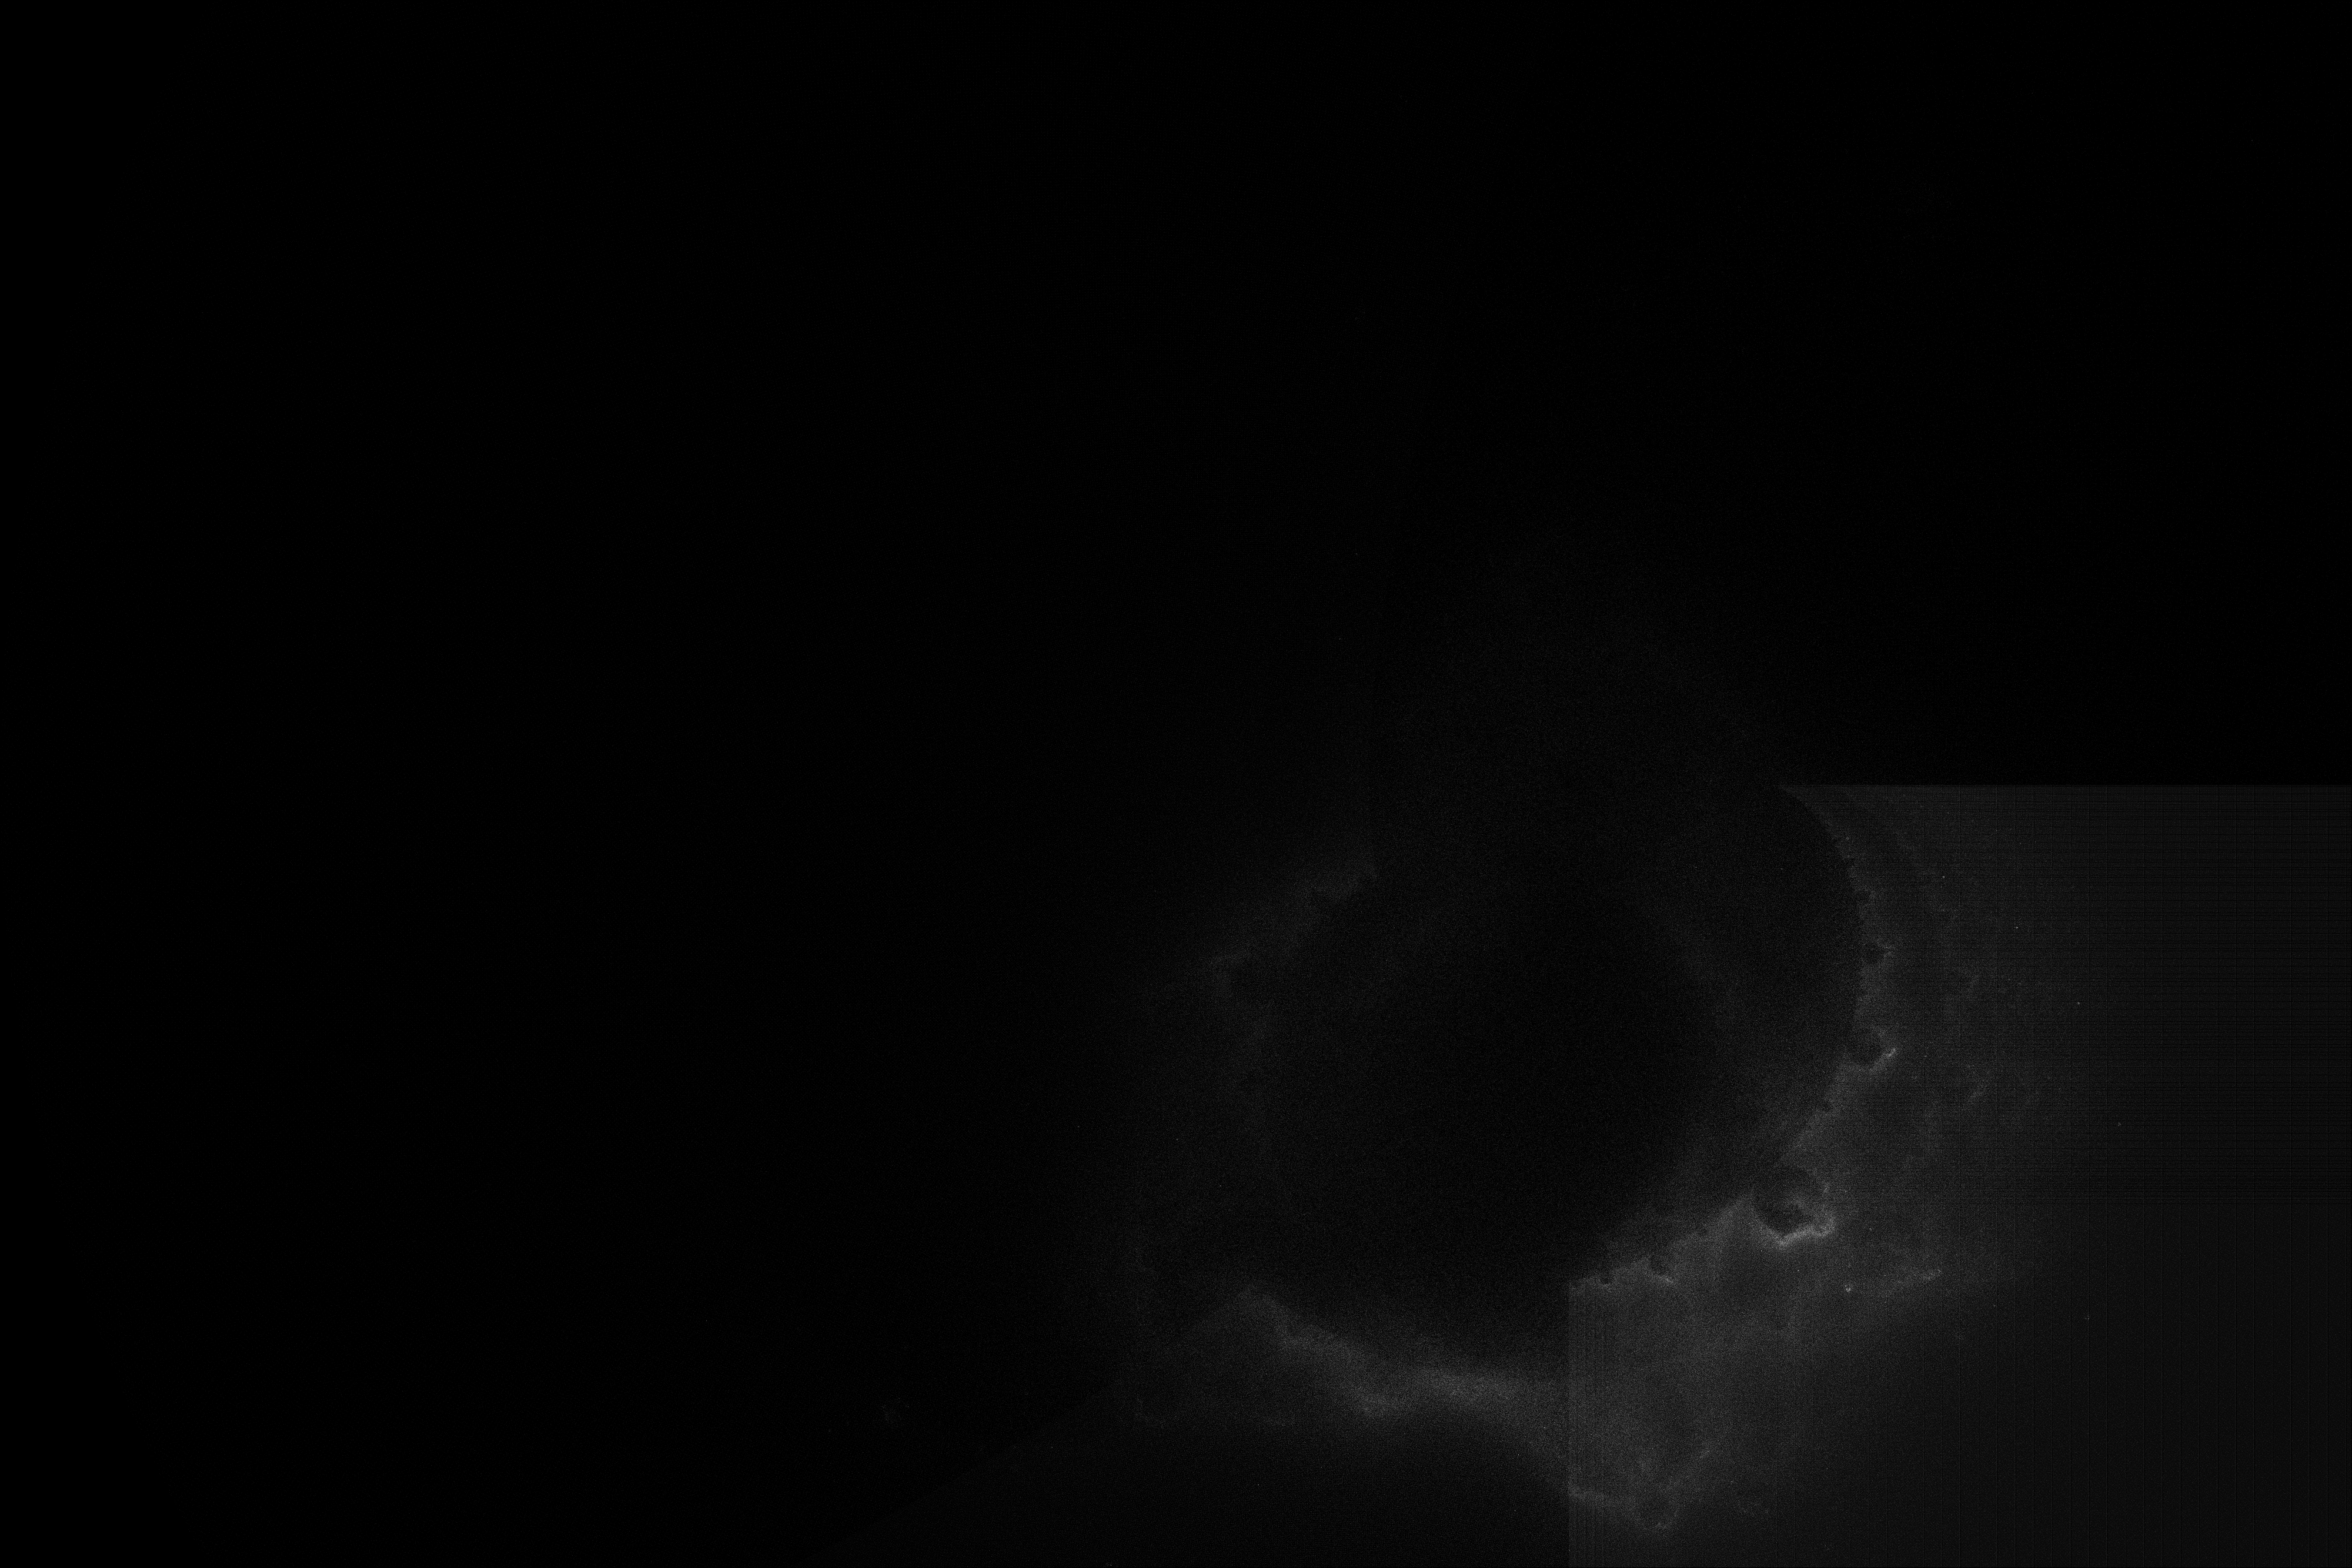
\includegraphics[width=.49\textwidth]{Pictures/1AnalyBuddhabrotmengeWithZoomGPU1ToPoint-0.5 + 0.0imWithIteration1000withResolution4000x2667.png}}\label{fig:1. Quadrant}}
	\hfill
	\subfloat[2. Quadrant]{\scalebox{1}[-1]{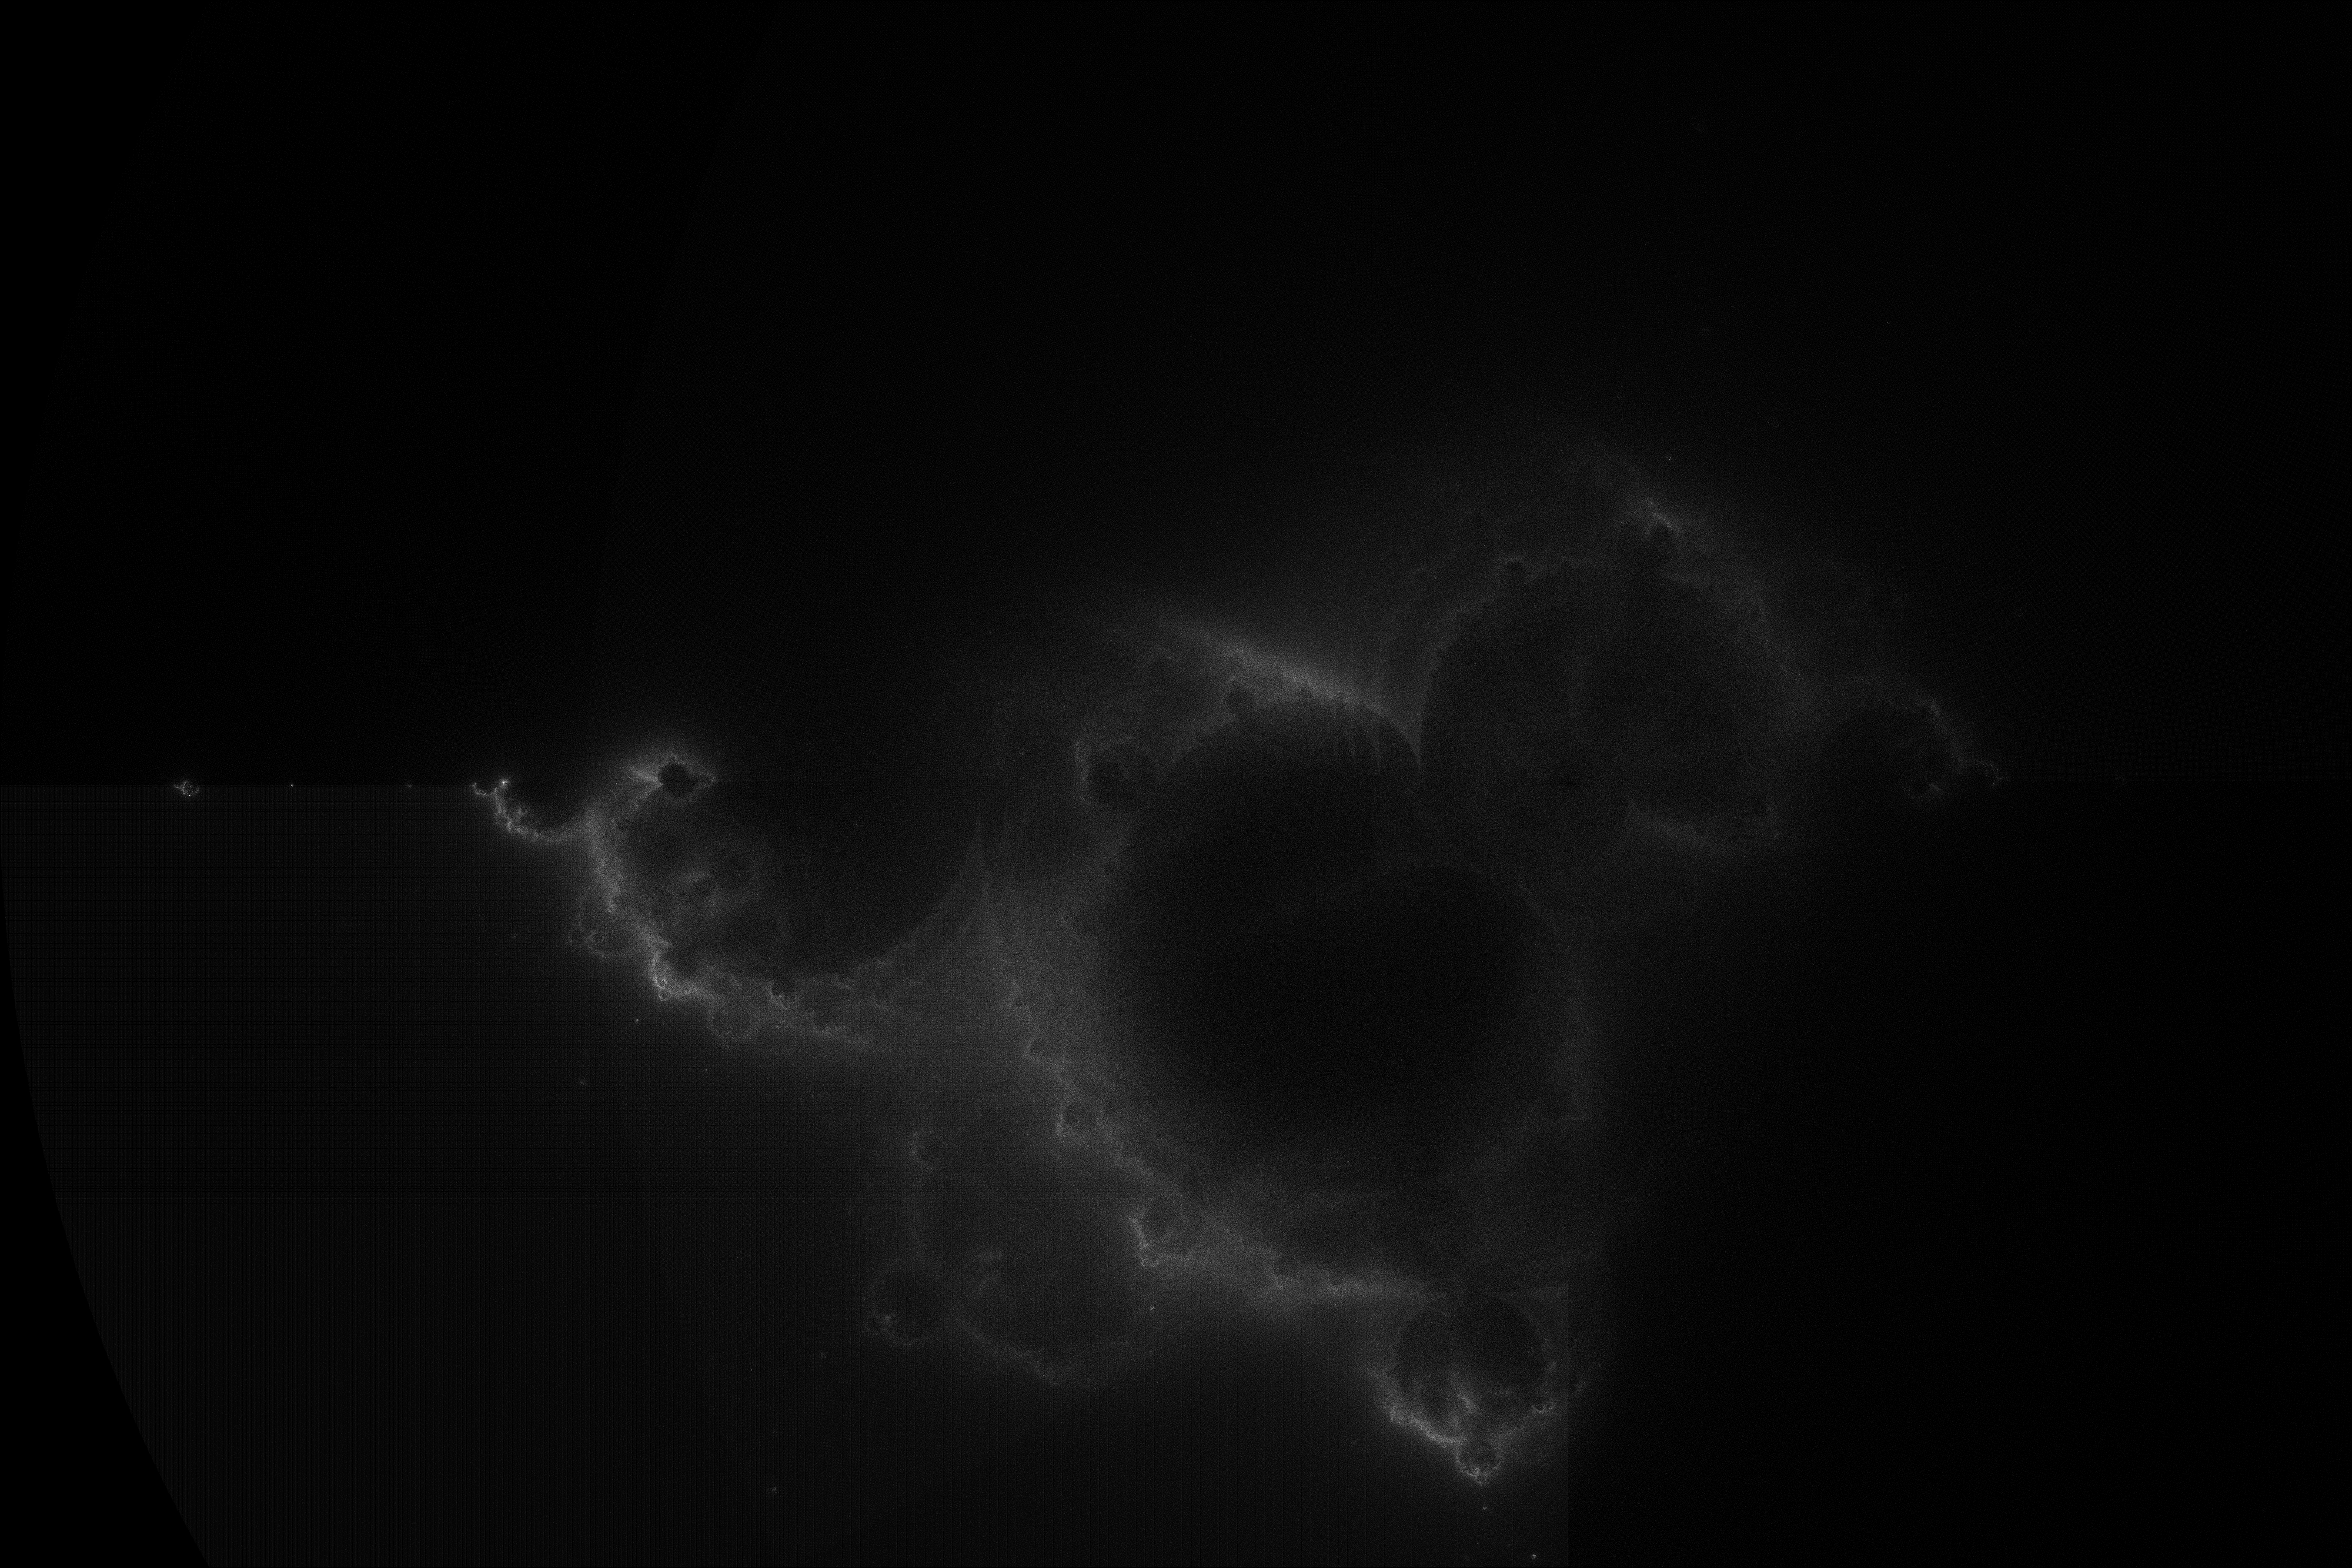
\includegraphics[width=.49\textwidth]{Pictures/2AnalyBuddhabrotmengeWithZoomGPU1ToPoint-0.5 + 0.0imWithIteration1000withResolution4000x2667.png}}\label{fig:2. Quadrant}}
	\caption{Die Enstehung der Kochkurve}
\
\end{figure}
\subsection{Implementierungszahlen}
Durch die gefunde Lösung ist zumal nurnoch einen 6.47-Facher Zoom möglich, dies wird daran liegen das es zwei Variabeln hat, welch ein kleiner einfluss ist, und dass nun grosse Matrixen in einer Liste zu finden sind, welches viel Speicherplatz nimmt. Es ist jedoch ein minimaler Verlust und somit nicht schlimm. Ein 6.47-Facher Zoom zum Punkt -1.5, mit der Auflösung 4'002 auf 2'668 Pixel und mit 1'000 Iteration nurnoch 1 Stunde 2 min 7 Sekunden.
